\documentclass[a4paper,12pt]{article} %style de document
\usepackage[utf8]{inputenc} %encodage des caractères
\usepackage[french]{babel} %paquet de langue français
\usepackage[T1]{fontenc} %encodage de la police
\usepackage[top=2cm,bottom=2cm,left=2cm,right=2cm]{geometry} %marges
\usepackage{graphicx} %affichage des images


\begin{document} %début du document



%----------------------------------
%page de garde
%----------------------------------

\begin{titlepage}

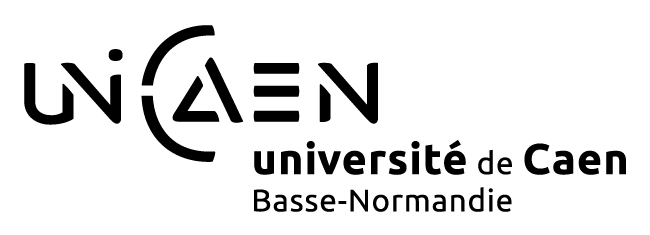
\includegraphics[scale=0.3]{images/unicaen.png}

\vspace{7cm}

\begin{center}

\begin{Huge}
Complément POO\\
Rapport du Devoir\\
\end{Huge}
\vspace{2cm}
\begin{large}
Beauchamp Aymeric 21301016\\
Chagneux Dimitri 21606807\\
Mori Baptiste 21602052\\
Leblond Valentin 21609038\\
\vspace{1cm}
L2-Info-groupe-4A
\end{large}

\end{center}
\end{titlepage}


%------------------------------
%sommaire
%------------------------------

\newpage

\tableofcontents{}

\newpage

%------------------------------
%contenu
%------------------------------


\section*{Introduction}
\addcontentsline{toc}{section}{Introduction}

L'objectif de ce projet de POO est de réaliser un taquin : un casse-tête consistant à déplacer des cases d'un plateau afin de les replacer dans l'ordre et ainsi reconstituer une image ou un motif donné.

\begin{figure}[!h]
\centering
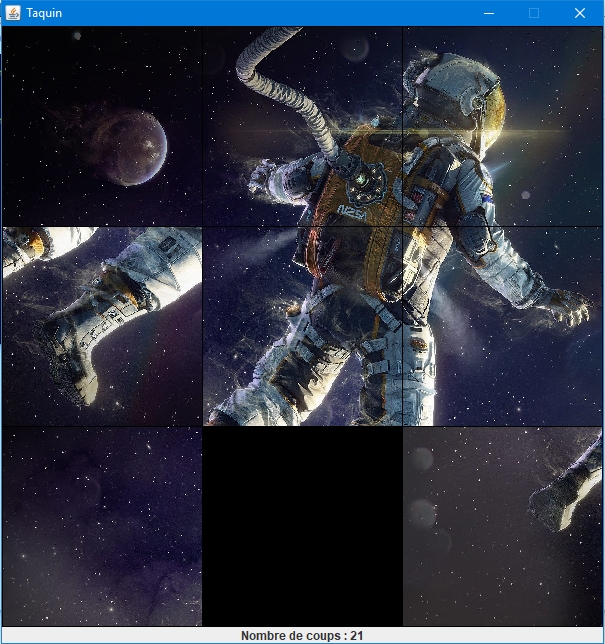
\includegraphics[scale=0.5]{images/Capture.PNG}
\caption{Jeu du Taquin}
\end{figure}

Nous avons séparé le projet en deux packages, le premier comportant le modèle du jeu utilisable en version console (le package \textbf{model}), et le deuxième, l'implémentation de l'interface graphique (le package \textbf{GUI}). Nous utilisons également un troisième dossier \textbf{ressources} où sont stockées les images utilisées par l'application.

\section{La conception du package model}

Le modèle de base du taquin est constitué d'une grille d'objets représentant les différentes cases. Les cases pleines ont des identifiants pour permettre de mettre en place la condition de victoire : on gagne si chaque identifiant est placé aux bonnes coordonnées.

\subsection{Organisation des classes}

Tout d'abord, nous avons représenté les cases par deux classes, \textit{\textbf{FullTile}} pour les cases pleines et \textit{\textbf{EmptyTile}} pour la zone vide qu'on déplacera. Ces classes possèdent des attributs en commun qui sont les coordonnées X et Y dans la grille ; c'est pourquoi nous avons conçu une classe abstraite \textit{Tile} qui possède ces coordonnées et dont héritent FullTile et EmptyTile.\\
La classe FullTile diffère de EmptyTile en ce qu'elle possède en plus un identifiant entier que l'on rend unique pour chaque instance utilisée.\\

Ensuite, nous avons une classe Board qui décrit l'état du jeu et le fait évoluer.

\begin{figure}[!h]
\centering
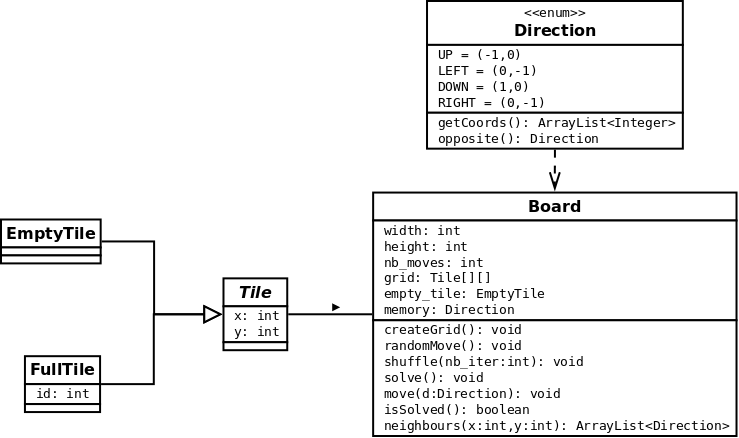
\includegraphics[scale=0.4]{images/model.png}
\caption{Diagramme de classe du package model}
\end{figure}

\newpage

\subsection{Fonctionnement du modèle}

Comme nous l'avons expliqué, l'initialisation et la mise à jour du modèle se font par le biais de la classe Board.\\

En premier lieu, nous avons une fonction \textbf{createGrid} qui permet d'initialiser une grille avec des FullTile et une EmptyTile et une fonction \textbf{toString} qui permet de l'afficher.\\
La grille ainsi créée est dans un état résolu où les identifiants des cases sont rangés dans l'ordre ci-dessous :

\begin{figure}[!h]
\centering
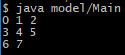
\includegraphics[scale=1]{images/Capture2.PNG}
\caption{Affiche d'une grille 3x3 initialisée}
\end{figure}

Puis, nous avons crée les déplacements de la case vide, nous avons d'abord commencer par créer une enum Direction avec quatre instances UP, DOWN, LEFT, RIGHT qui représentent une direction de déplacement. Nous utilisons cette enum dans la fonction \textbf{move} qui déplace la case vide dans la direction donnée en argument.\\

Pour mélanger le jeu, on choisit un mouvement aléatoire selon les mouvements possibles de la case vide puis on déplace la case vide jusqu'en bas à droite, à sa position initiale. On garde en mémoire le dernier coup effectué afin d'éviter des coups inutiles qui réduisent l'efficacité du mélange ; si l'on va vers le haut lors d'un coup, on interdit d'aller vers le bas au coup suivant.\\
Le mélange est effectué par la fonction \textbf{shuffle} qui prend en argument le nombre de coups à réaliser avant de considérer le mélange comme terminé. Dans la version finale, nous faisons 10 000 mélanges. Cela assure une bonne dispersion des cases pour un temps de calcul négligeable.\\
Comme la grille initiale est résolue, l'état obtenu par le mélange n'est pas bloquant puisqu'il existe une séquence de coups menant de cet état à la solution.\\

La récupération des coups jouables de la case vide est un voisinage de taille 4 de rayon 1 qui correspond aux quatre directions haut, bas, gauche, droite. La fonction \textbf{neighbours} donne selon une coordonnée dans la grille du jeu donne toutes les directions possibles.\\

Le modèle dispose aussi d'une fonction \textbf{solve} qui résout le puzzle. Nous avons utilisé une approche extrêmement simple consistant à jouer un coup aléatoire jusqu'à obtenir la configuration initiale de la grille.\\
Cette simplicité a un coût : le solveur peut réaliser jusqu'à 500 000 coups pour résoudre un simple puzzle 3x3, et devient très lent dès que l'on veut augmenter la taille.
Nous sommes conscients qu'il est possible de réaliser un solveur plus efficace, par exemple via l'utilisation de l'algorithme A*, mais nous avons préféré ne pas nous focaliser sur cet aspect du projet.\\

La classe principale permet de jouer au taquin en interface console. Le joueur peut déplacer la case vide avec Z,Q,S,D.

\section{Conception du package GUI}

\subsection{Organisation des classes}


\subsection{Fonctionnement GUI}

D'abord, pour représenter l'état du jeu, la classe \textbf{View} permet à partir d'un chemin, d'une image et d'un Board découper l'image et lier

\end{document}
